\ifdefined\ANONBUILD
\documentclass[sigconf,anonymous,review]{acmart}
\else
\documentclass[sigconf,review]{acmart}
\fi

\usepackage{amsmath}
\usepackage{booktabs}
\usepackage{placeins}
\usepackage{tabularx}
\newif\ifanonymoussubmission
\ifdefined\ANONBUILD
  \anonymoussubmissiontrue
\else
  \anonymoussubmissionfalse
\fi

\newcommand{\system}{TRACE-RPG}
\newcommand{\Valid}{\mathrm{valid}}
\newcommand{\AcceptSet}{\mathcal{A}}
\newcommand{\GoalSet}{\mathcal{G}}
\newcommand{\HitSet}{\mathcal{H}}
\newcommand{\SchemaSet}{\mathcal{S}}
\newcommand{\RepoURL}{\ifanonymoussubmission [Anonymous Repository URL withheld for double-anonymous review]\else \url{https://github.com/akillness/neural_symbolic_in_game}\fi}
\AtBeginDocument{\emergencystretch=2.5em}
\providecommand{\Description}[2][]{}


\setcopyright{none}
\acmConference[AAMAS '27]{International Conference on Autonomous Agents and Multiagent Systems}{2027}{\ifanonymoussubmission Anonymous Submission\else Seoul, Republic of Korea\fi}

\begin{document}

\title{TRACE-RPG: Action-Shielding Proposal-to-Commit Boundaries and Counterexample Repair for Agentic Games}

\author{Jangyoung Jeong}
\affiliation{\institution{Department of Game Design, Hongik University}\city{Seoul}\country{Republic of Korea}}
\author{Shinjin Kang}
\authornote{Corresponding author.}
\affiliation{\institution{Hongik University}\city{Seoul}\country{Republic of Korea}}

\begin{abstract}
Autonomous LLM agents in interactive environments can produce schema-valid proposals that violate reachability, epistemic, or disclosure constraints. \system{} integrates a deterministic seven-predicate action shield, bottom-up transitive Datalog closure (\texttt{nesy\_game.multihop}), and state-blind counterexample repair $\rho(a,E)$ at the proposal-to-commit boundary (Theorems~1--4). Beyond 1,664 finite-graph boundary checks (260/416 $\rightarrow$ 0/416 unsafe) and 480 $R{\le}64, d{\le}5$ Datalog scaling checks (100.0\% at $\le$7.12\,$\mu$s median latency vs.\ 46.67\% flat and 60.00\% 2-hop, $Q{=}1100.19$), we evaluate \textbf{105 independent 5-turn closed-loop multi-agent episodes} (\textbf{P15}) using direct HTTPS Anthropic Claude~5.5 structured outputs across Haiku~5.5, Sonnet~5.5, and Opus~5.5 (omitting \texttt{temperature} where deprecated on Claude~5.5; \textbf{105/105} fresh 0-LLM trace replays exact): controlled Safe-RL proxy masking (0/15 safe goals, 1/15 zero-leak, 16/61 unsafe turns) and NeMo-style Colang proxy rails (1/15, 1/15, 15/61) miss multi-hop leaks, whereas \system{} achieves \textbf{15/15 (100.0\%)} zero-leak and \textbf{0} unsafe commits across every multihop arm (confirming Theorem~2 no-op safety with $\rho_{\mathrm{repairs}}{=}0$ on 28 state-dependent rejections across 14/15 \texttt{rho\_k2} and 13/15 \texttt{multihop\_k0}, and reaching \textbf{15/15 (100.0\%)} safe goals via $\rho{+}\text{LLM}_{K=1}$; $Q_{\mathrm{goal}}{=}68.71$, McNemar $p{\le}1.22{\times}10^{-4}$). Attested API factorial runs (\textbf{P16A}: 60 episodes, \texttt{ontology\_multihop} 30/30 zero-leak, 22 $\rho$ repairs, and 11/30 goals vs.\ \texttt{general\_rule} 22/30 and 0/30, $p{=}0.00781$), Godot~4.7.1 executions (\textbf{P16B}: 21/21 exact replays, 6/6 \texttt{SealedLighthouse} terminal hashes), cross-family CLI trials (\textbf{P11}--\textbf{P13}: GPT-OSS~120B + Hydrogen~4, 0/79 and 0/84 unsafe, $(a,E)$ repair 27/27 vs.\ 26/27 at 0 extra tokens), and 540 unified EN/KO escape checks (\textbf{P17}: $\kappa{=}0.8813$, 0\% FRR) establish reproducible multi-agent safety.
\end{abstract}

\begin{CCSXML}
<ccs2012>
   <concept>
       <concept_id>10010147.10010178.10010219.10010221</concept_id>
       <concept_desc>Computing methodologies~Intelligent agents</concept_desc>
       <concept_significance>500</concept_significance>
   </concept>
   <concept>
       <concept_id>10010147.10010178.10010187</concept_id>
       <concept_desc>Computing methodologies~Knowledge representation and reasoning</concept_desc>
       <concept_significance>300</concept_significance>
   </concept>
</ccs2012>
\end{CCSXML}

\ccsdesc[500]{Computing methodologies~Intelligent agents}
\ccsdesc[300]{Computing methodologies~Knowledge representation and reasoning}

\keywords{action shielding, neuro-symbolic agents, counterexample-guided repair, epistemic disclosure}

\maketitle

\section{Introduction}
Generated game events can satisfy a syntactic schema and cite known facts while requesting inaccessible objects, unauthorized state transitions, or premature secret disclosure. Grounding and plausible dialogue \cite{S03_weir2024ontologically,S20_ashby2023personalized} supply candidate content, yet the game engine must still decide which state transitions to authorize.

\system{} enforces this decision at an external proposal-to-commit boundary (Fig.~\ref{fig:architecture}). Models and adapters submit typed candidates to a deterministic gate that checks action policies, preconditions, object reachability, NPC knowledge, disclosure permissions, effects, and quest-stage monotonicity. When a check fails, the gate returns structured errors for bounded repair; repair modifies only the candidate rather than canonical state, and mutation occurs only after same-state revalidation. A read-only eight-role ontology view links source declarations to these checks and public decisions without write authority, while hash-linked transition records support semantic replay and assignment-complete accounting.

Conceptually, this contract goes beyond factual grounding by separating an NPC's \emph{epistemic knowledge boundary} (facts an actor knows) from its \emph{disclosure authorization policy} (facts an actor may reveal at the current quest stage). Methodologically, our evaluation separates a zero-LLM-call deterministic verification layer (gate checks, guided repair, and engine replay) from a bounded stochastic proposer layer with explicit failure retention.

Across deterministic audits, a schema-only baseline committed 260/416 reference-invalid proposals across 32 finite-graph configurations, whereas all semantic-gate arms recorded \textbf{0/416} unsafe commits, 0/156 false rejections, and 128/260 $\rho$ repairs, while 480 $R{\le}64, d{\le}5$ procedural Datalog checks (\textbf{P9}) established 100.0\% oracle parity at $\le$7.12\,$\mu$s median latency vs.\ 46.67\% flat and 60.00\% 2-hop ($Q{=}1100.19$). Extending Theorems~1--4 for invariants \textbf{I1--I4}, attested direct HTTPS Anthropic Claude~5.5 API evaluations across Haiku, Sonnet, and Opus~5.5 confirm \textbf{0} unsafe commits across 105 independent 5-turn closed-loop trajectories (\textbf{P15}: 15/15 zero-leak vs.\ Safe-RL~\cite{alshiekh2018shield} 1/15 and NeMo-style~\cite{rebedea2023nemo} 1/15 proxy rails, 15/15 hybrid safe goals), 60 prospective factorial episodes (\textbf{P16A}: \texttt{ontology\_multihop} 30/30 zero-leak and 22 repairs vs.\ 22/30 \texttt{general\_rule}), 21 Godot~4.7.1 closed-loop episodes (\textbf{P16B}: 21/21 exact replays, 6/6 \texttt{SealedLighthouseMachine} terminal hashes), and 540 unified EN/KO escape checks (\textbf{P17}: $\kappa{=}0.8813$, 0\% FRR), alongside cross-family CLI tracks (\textbf{P11}--\textbf{P14}: $(a,E)$ repair 27/27 vs.\ 26/27 at 0 extra tokens), \texttt{DATASHEET\_v5.md}~\cite{gebru2021datasheets}, Croissant~1.0 v5~\cite{akhtar2024croissant} (26/26 SHA-256 digests), and quarantined \texttt{TR01--TR06} ($N{=}0$, \texttt{AWAITING\_HUMAN\_RATERS}).

\section{Related Work and Research Gap}
Grounding, memory, planning, and role-based agents \cite{S03_weir2024ontologically,S20_ashby2023personalized,S07_park2023generative,S08_shao2023character}, together with player and dialogue systems \cite{S21_akoury2023player,S22_hochreiter2026beyond,S23_yin2026contextualized,S02_figueiredo2025scaffolded}, support contextual interaction, whereas we examine whether the current encoded state and disclosure policy permit a proposed transition. Modeling affect and engagement \cite{S24_yannakakis2011experiencedriven,S25_melhart2020engagement,S26_wang2026engagement} targets different outcomes: style preferences, affect estimates, and personality labels may guide generation but do not authorize state mutations.

Existing benchmarks and automated play-testing cover state, embodiment, content, process, social interaction, and long-horizon play \cite{S11_cote2019textworld,S12_wang2022scienceworld,S13_fan2022minedojo,S14_perezliebana2019gvgai,S15_liu2024agentbench,S16_ma2024agentboard,S17_zhou2024sotopia,S18_paglieri2025balrog,S19_lepelletier2022playtesting}, while NCP-Bench evaluates narrative commitment and fact consistency \cite{S58_ma2026ncpbench}. Structural, schema, affordance, and neuro-symbolic rule methods motivate our constraint design \cite{S09_geng2023grammar,S10_beurerkellner2023prompting,S36_scholak2021picard,S50_kambhampati2024llmmodulo,S51_ichter2023saycan,S52_wang2025agentspec,S53_li2025settingdc,S54_zhou2025story2game,S42_buongiorno2024pangea,alshiekh2018shield,rebedea2023nemo}, alongside counterexample-guided repair \cite{S45_madaan2023selfrefine,S48_shinn2023reflexion,S46_chen2023selfdebug,S47_solarlezama2006sketching} and reproducibility/accounting standards \cite{S31_agarwal2021precipice,S33_pineau2021reproducibility,S56_feng2025agentrr,S59_sun2025bdc,gebru2021datasheets,akhtar2024croissant}. Unlike prior systems that conflate schema validity with action legality or treat factual grounding as sufficient for dialogue safety, \system{} isolates schema parsing, epistemic knowledge, disclosure permission, and canonical state commit into separately auditable gates.


\begin{figure*}[!t]
  \centering
  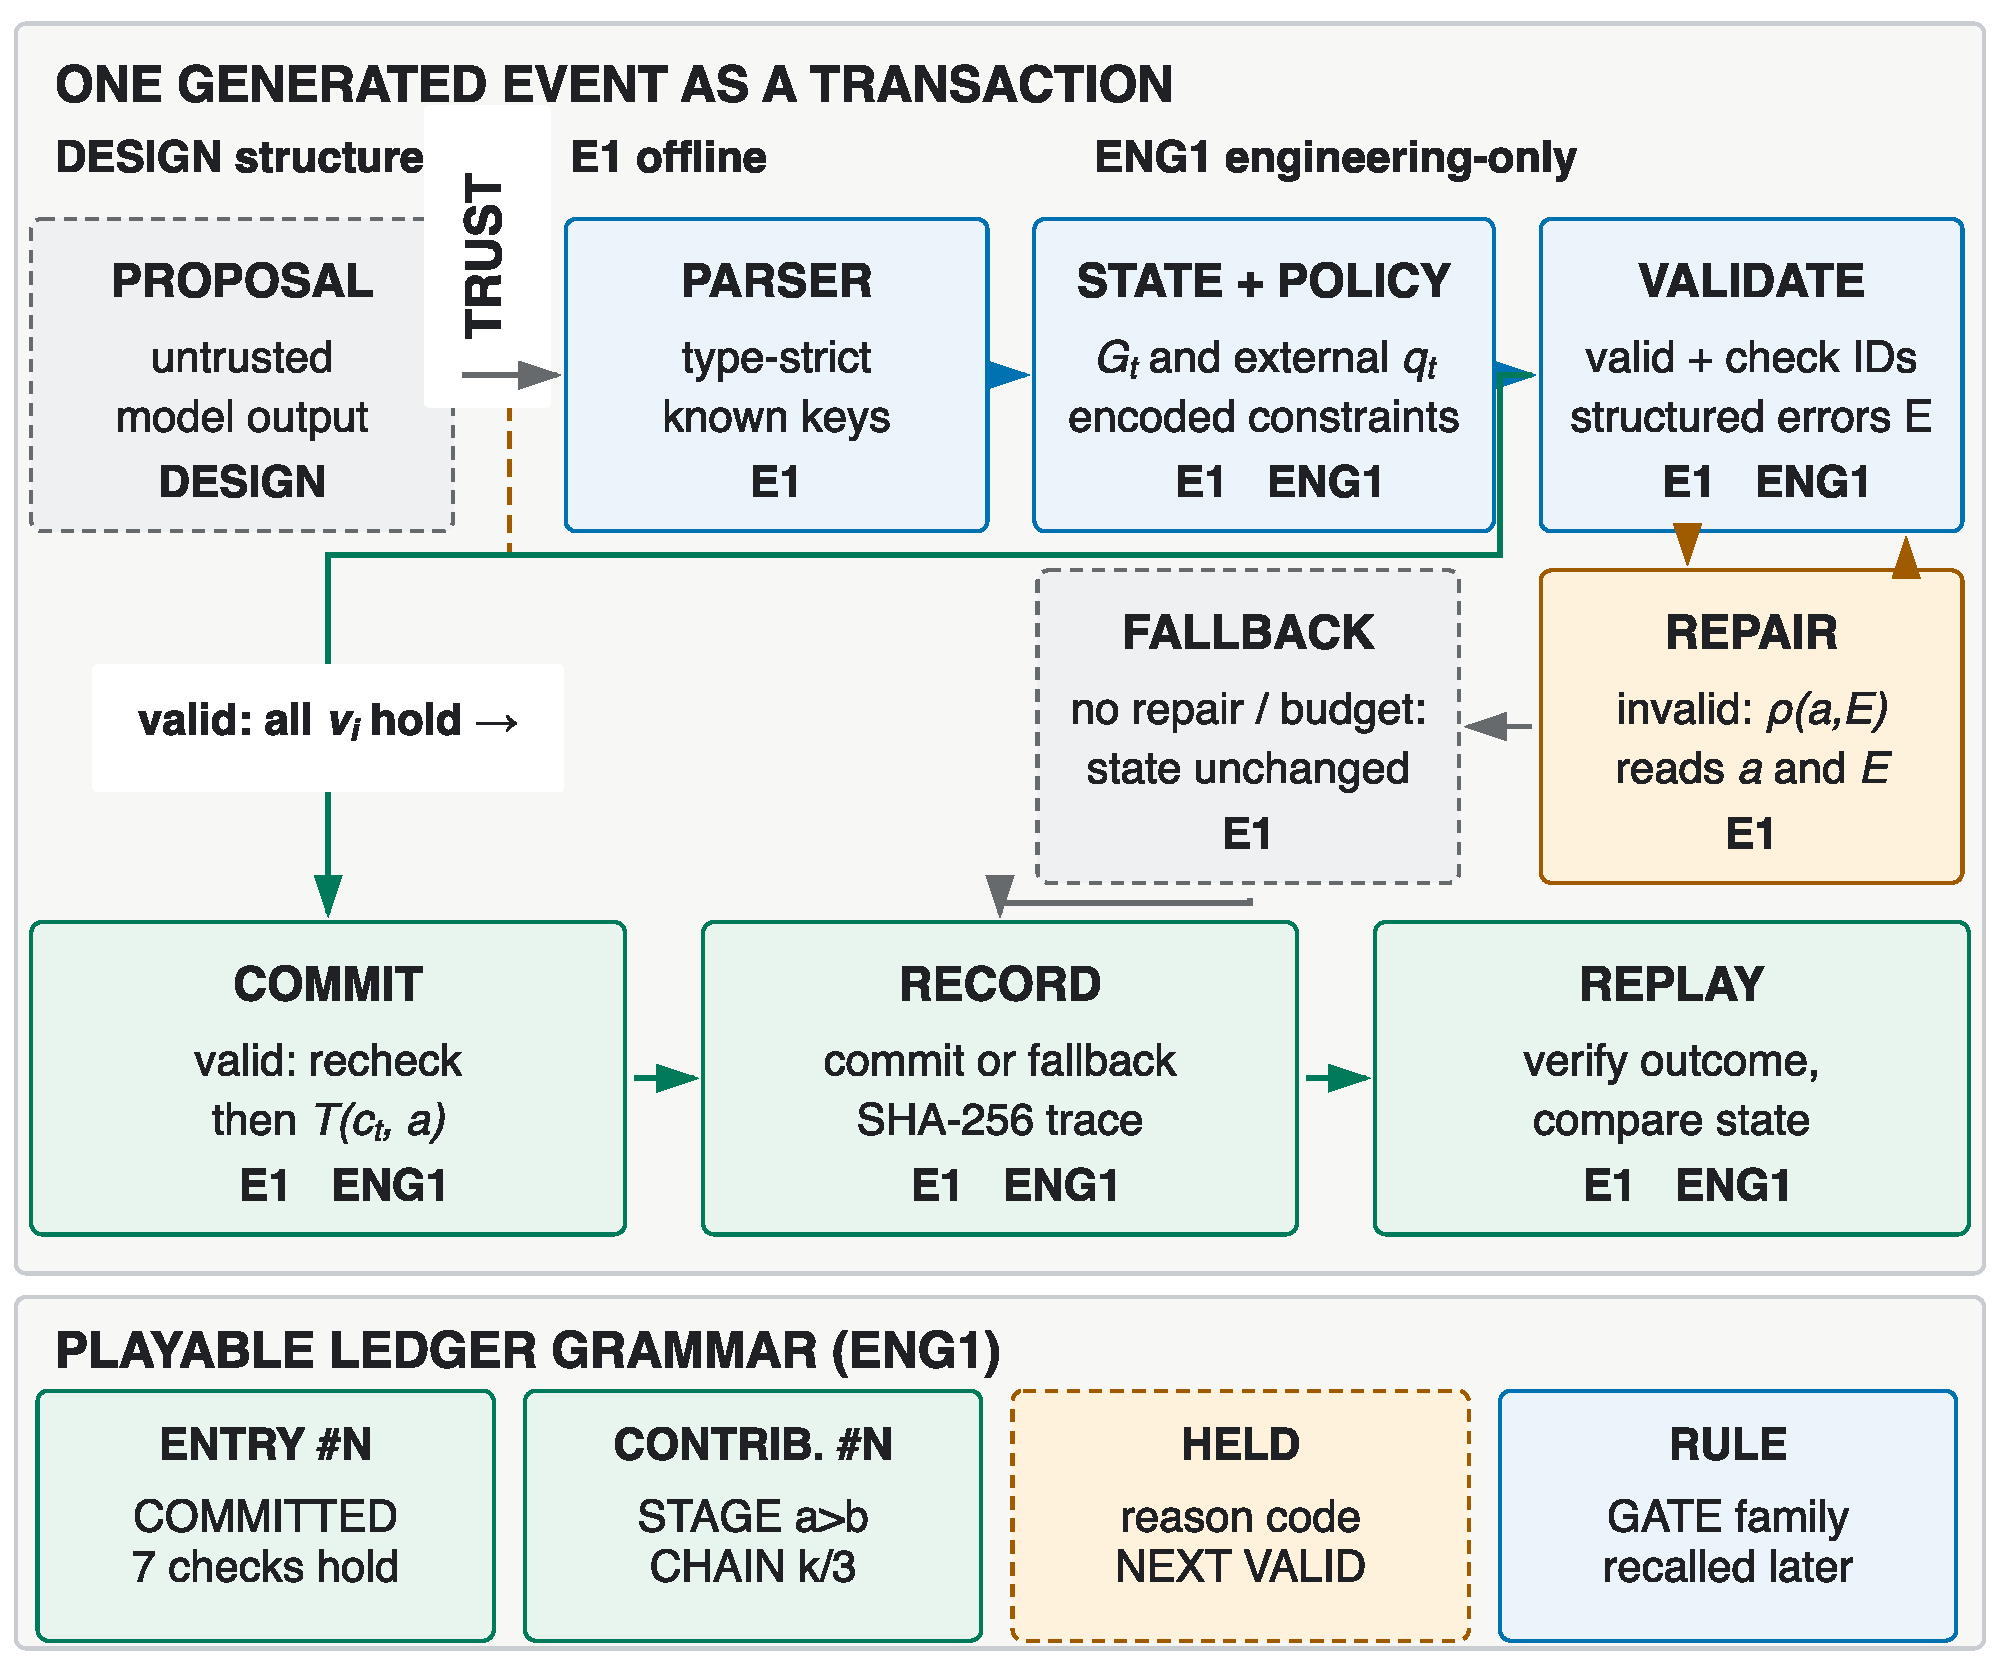
\includegraphics[width=0.72\textwidth]{../../figures/fig_architecture.pdf}
  \caption{Policy and state $c_t$ shield proposals; errors feed bounded $\rho$ or unchanged fallback before revalidated commit and replay.}
  \Description{Architecture diagram showing proposal submission, seven-predicate deterministic shielding, bounded repair, revalidation, and commit ledger.}
  \label{fig:architecture}
\end{figure*}

\section{Problem Definition and Guarantee Boundary}\label{sec:problem}
In $c_t=(G_t,q_t)$, $G_t$ denotes the typed game snapshot (locations, reachable locations, object placements, inventory, facts, NPC knowledge, and quest stage) and $q_t$ contains externally authored action-policy, disclosure, and quest-stage constraints. Predicates neither reconstruct history $h_{<t}$ nor mutate $q_t$, and retrieval outputs or affect scores carry zero write authority.

After strict schema parsing of an untrusted proposal $a_t$, the validator runs seven deterministic predicates and returns \texttt{Validation}\allowbreak\texttt{Result}(\allowbreak$\mathrm{valid},E_t,C_{\mathrm{run}}$):
\begin{equation}
\begin{aligned}
V(c_t,a_t)&=(\mathrm{valid},E_t,C_{\mathrm{run}}),\\
\boldsymbol{v}&=(v_{\mathrm{policy}},v_{\mathrm{pre}},v_{\mathrm{reach}},\\
&\qquad v_{\mathrm{know}},v_{\mathrm{disc}},v_{\mathrm{elig}},v_{\mathrm{stage}})\in\{0,1\}^{7},
\end{aligned}
\end{equation}
where $\mathrm{valid}\equiv\bigwedge_{i=1}^{7}(v_i=1)$ and $E_t$ records typed error codes, entities, reasons, and repair hints. Canonical state updates only when all seven predicates pass:
\begin{equation}
c_{t+1}=\begin{cases}
T(c_t,a_t), & \bigwedge_{i=1}^{7}(v_i=1),\\
c_t, & \text{otherwise.}
\end{cases}
\label{eq:transition}
\end{equation}

\subsection{Schema Validity, Authorization, and Goal Success}\label{sec:authorization-sets}
Fix the pre-action state $c_t$, authored policy, and strict schema. Let $\SchemaSet$ be the set of schema-valid candidates; we separate authorization from goal attainment:
\begin{equation}
\begin{aligned}
\AcceptSet(c_t)&=\{a\in\SchemaSet:V(c_t,a).\mathrm{valid}\},\\
\GoalSet(c_t)&=\{a\in\SchemaSet:\operatorname{Goal}(T(c_t,a))\},\\
\HitSet(c_t)&=\AcceptSet(c_t)\cap\GoalSet(c_t)\subseteq\AcceptSet(c_t)\subseteq\SchemaSet.
\end{aligned}
\end{equation}
A schema-valid candidate that declares a forbidden fact falls outside $\AcceptSet$, whereas a permitted observation action can lie inside $\AcceptSet$ yet outside $\GoalSet$. Knowledge and disclosure permission are independent inputs: an NPC can know \texttt{keeper\_\allowbreak secret} at both stage $0$ and stage $1$ while disclosure is forbidden at stage $0$ and permitted at stage $1$.

\subsection{Formal Security Theorems for Invariants I1--I4}\label{sec:formal-proofs}
Under Eq.~\eqref{eq:transition} and strict parser \texttt{parse\_}\allowbreak\texttt{candidate\_}\allowbreak\texttt{mapping}, invariants \textbf{I1--I4} hold as conditional structural theorems over any finite encoded state $c_t=(G_t,q_t)$, repair budget $K\in\mathbb{Z}_{\geq 0}$, and returning callbacks:

\noindent\textbf{Theorem 1 (I1: State-Preservation Safety).} \emph{If the initial candidate fails strict parsing or all $K{+}1$ candidates yield $V(c_t,a^{(j)}).\mathrm{valid}=\mathrm{false}$, then $c_{t+1}=c_t$ and committed effects are empty.}
\par\noindent\textit{Proof.} \texttt{parse\_}\allowbreak\texttt{candidate\_}\allowbreak\texttt{mapping} rejects malformed proposals prior to commit; in Fig.~\ref{alg:commit}, $\operatorname{Commit}$ is reachable only on $\mathrm{ok}=\mathrm{true}$, while $j=K$ invokes $\operatorname{Fallback}(c_t)$ returning $c_t$ untouched by Eq.~\eqref{eq:transition}. \hfill$\square$

\noindent\textbf{Theorem 2 (I2: Bounded Termination and State-Blind Anti-Laundering Repair).} \emph{For any finite $K{\geq}0$ and returning callbacks, the loop executes at most $K{+}1$ validator calls, revalidates $V(c_t,a^{(j)})$ immediately prior to mutation, and never alters \texttt{WorldState}-dependent authorization classes under $\rho$.}
\par\noindent\textit{Proof.} Loop counter $j$ starts at $0$, checks $j=K$ before incrementing, and halts on $\mathrm{ok}=\mathrm{true}$ or $j=K$, bounding $V$ calls by $K{+}1$. By Table~\ref{tab:rho-rules}, $\rho(a,E)$ inspects only $(a,E)$ without reading \texttt{WorldState} and maps \texttt{UNKNOWN\_}\allowbreak\texttt{ACTION\_}\allowbreak\texttt{TYPE}, \texttt{UNREACHABLE\_}\allowbreak\texttt{REQUIRED\_}\allowbreak\texttt{OBJECT}, \texttt{NPC\_}\allowbreak\texttt{KNOWLEDGE\_}\allowbreak\texttt{VIOLATION}, \texttt{NPC\_}\allowbreak\texttt{DIS\-CLOSURE\_}\allowbreak\texttt{KNOW\-LEDGE\_}\allowbreak\texttt{VIO\-LATION}, \texttt{FORBIDDEN\_}\allowbreak\texttt{DISCLOSURE}, \texttt{QUEST\_}\allowbreak\texttt{STAGE\_}\allowbreak\texttt{VIOLATION}, and \texttt{QUEST\_}\allowbreak\texttt{STAGE\_}\allowbreak\texttt{REGRESSION} to identity while dropping same-field conflicts. \hfill$\square$

\noindent\textbf{Theorem 3 (I3: Policy-Bounded Mutation).} \emph{Every committed state transition satisfies all seven predicates $v_1\dots v_7$ and applies only effects permitted by \texttt{ActionPolicy.}\allowbreak\texttt{allowed\_}\allowbreak\texttt{effects}.}
\par\noindent\textit{Proof.} Strict parsing freezes the 12 \texttt{CANDIDATE\_}\allowbreak\texttt{FIELDS}; $v_{\mathrm{policy}}{=}1$ verifies effect membership in \texttt{allowed\_}\allowbreak\texttt{effects} and $T$ writes no undeclared keys. \hfill$\square$

\noindent\textbf{Theorem 4 (I4: Deterministic Semantic Replay).} \emph{Given ordered hash-chained transition records with \texttt{allow\_}\allowbreak\texttt{defaults=false} parsing and frozen $(V,T)$, replaying proposals from $c_0$ uniquely reconstructs $c_T$ and detects any single-step tampering via SHA-256 chain mismatch.}
\par\noindent\textit{Proof.} Both $V$ and $T$ are pure deterministic functions of $(c_t,a_t)$, and each record hashes $(\mathrm{hash}(c_t),\allowbreak a_t,\allowbreak V(c_t,a_t),\allowbreak\mathrm{hash}(c_{t+1}))$; inductive agreement from $c_0$ yields $\mathrm{hash}(c'_T)=\mathrm{hash}(c_T)$. \hfill$\square$

\section{TRACE-RPG Architecture and Algorithms}\label{sec:arch}
Models and adapters submit typed candidate JSON via direct HTTPS structured decoding or constrained prompts, the strict parser rejects unknown keys and ambiguous types, and a versioned bridge exchanges observations, candidates, validation errors, repairs, and commits (Fig.~\ref{fig:architecture}, Table~\ref{tab:validators}). An eight-role read-only ontology view (\texttt{World}, \texttt{Actor}, \texttt{Knowledge}, \texttt{Fact}, \texttt{Policy}, \texttt{Quest}, \texttt{Action}, \texttt{Trace}) links source declarations to executed predicates without write authority.

\subsection{Multi-Hop Datalog Closure and Comparative Safety Baselines}\label{sec:multihop-baselines}
When narrative secrets derive through multi-step premise chains or role hierarchies up to depth $d$, flat 1-hop gating fails to detect indirect leaks. The core \texttt{nesy\_\allowbreak game.\allowbreak multihop} module evaluates a frozen declarative \texttt{MultihopOntologySpec} containing \texttt{role\_parents}, \texttt{fact\_implications}, \texttt{forbidden\_by\_role}, and \texttt{min\_stage\_by\_fact}. Calling \texttt{compute\_datalog\_closure} computes the bottom-up semi-naive fixpoints over role inheritance $\mathcal{R}^*(u)$ and fact implications $\mathcal{F}^*(S)$ up to arbitrary finite depth $d$:
\begin{equation}
\mathcal{F}^*(S)=\operatorname{lfp}\Big(X\mapsto S\cup\bigcup_{f\in X}\texttt{fact\_implications}(f)\Big),
\end{equation}
and propagates role prohibitions $\bigcup_{r\in\mathcal{R}^*(u)}\texttt{forbidden\_by\_role}(r)$ plus dynamic state prohibitions before evaluating $v_{\mathrm{know}}, v_{\mathrm{disc}}, v_{\mathrm{stage}}$ in \texttt{validate\_\allowbreak candidate\_\allowbreak multihop}. To situate this boundary against established safety paradigms over the identical \texttt{WorldState} contract without external neural RL policy training or separate server deployments, our package implements two controlled in-engine proxy comparators: (i)~\textbf{Safe-RL Action Masking} (\texttt{evaluate\_\allowbreak action\_\allowbreak mask\_\allowbreak shield}, following~\cite{alshiekh2018shield}), which enforces declared action-type, reachability, and 1-hop precondition masks over observable action tuples while omitting transitive role/fact closure; and (ii)~\textbf{NeMo-style Colang Output Rail} (\texttt{evaluate\_\allowbreak dialog\_\allowbreak rail\_\allowbreak filter}, following~\cite{rebedea2023nemo}), which filters surface secret strings and direct 1-hop dialogue policies over emitted utterances without multi-hop state closure.

\begin{table}[!tbp]
\caption{Encoded Seven-Predicate Validator Boundary}
\label{tab:validators}
\centering
\footnotesize
\begin{tabularx}{\columnwidth}{@{}>{\raggedright\arraybackslash}p{0.25\columnwidth}>{\raggedright\arraybackslash}X>{\raggedright\arraybackslash}p{0.17\columnwidth}@{}}
\toprule
\textbf{Predicate} & \textbf{Rejects} & \textbf{On failure} \\
\midrule
Action policy & unknown action/type; omitted preconditions/effects; disallowed effects & unchanged \\
Precondition & absent or false requirement & unchanged \\
Reachability & inaccessible target object & unchanged \\
NPC knowledge & used/disclosed fact absent from actor knowledge & unchanged \\
Disclosure & declared or Datalog-derived forbidden fact & unchanged \\
Quest stage & required stage (incl.\ derived min-stage) above current stage & unchanged \\
Stage monotonicity & regressive quest-stage mutation & unchanged \\
\bottomrule
\end{tabularx}
\end{table}

\begin{figure}[!tbp]
\centering
\footnotesize
\begin{tabular}{@{}rl@{}}
1: & $a\leftarrow\operatorname{Propose}(c)$; $j\leftarrow0$ \\
2: & \textbf{repeat} \\
3: & \quad $(\mathrm{ok},E)\leftarrow V(c,a)$; $\operatorname{Record}(a,E)$ \\
4: & \quad \textbf{if} $\mathrm{ok}$ \textbf{then assert} $V(c,a).\mathrm{ok}$; \textbf{return} $\operatorname{Commit}(c,a)$ \\
5: & \quad \textbf{if} $j=K$ \textbf{then return} $\operatorname{Fallback}(c)$ \\
6: & \quad $a\leftarrow\operatorname{Repair}(c,a,E)$; $j\leftarrow j+1$ \\
7: & \textbf{until terminal}
\end{tabular}
\caption{Validate--Repair--Commit records at most $K+1$ candidate attempts and revalidates before mutation.}
\Description{Pseudocode of the Validate-Repair-Commit loop bounding validator calls to K+1 and revalidating prior to commit.}
\label{alg:commit}
\end{figure}

Guided repair $\rho(a,E)=a\oplus\bigcup_{e\in E}\delta(e)$ (Fig.~\ref{alg:commit}, Table~\ref{tab:rho-rules}) and \texttt{execute\_\allowbreak with\_\allowbreak multihop\_\allowbreak repair} inspect only candidate $a$ and typed errors $E$, never \texttt{WorldState}, preventing state laundering on authorization faults. Transition records chain unkeyed SHA-256 hashes over prior state, candidate, validation outcome, and recomputed final state for bit-exact semantic replay.

\begin{table}[!tbp]
\caption{Per-Error-Class Edits of Guided Repair $\rho(a,E)$}
\label{tab:rho-rules}
\centering
\footnotesize
\begin{tabularx}{\columnwidth}{@{}>{\raggedright\arraybackslash}X>{\raggedright\arraybackslash}X@{}}
\toprule
\textbf{Validator error class} & \textbf{Edit $\delta(e)$ on candidate $a$} \\
\midrule
Policy precondition / effect omission & insert named predicate or effect \\
Policy effect violation & drop disallowed effect \\
Unsatisfied precondition & drop named predicate \\
Unauthorized stage mutation & clear \texttt{quest\_stage\_effect} \\
Unknown action; reachability, knowledge, disclosure, or stage classes & no-op (prevents state laundering) \\
\bottomrule
\end{tabularx}
\end{table}

\section{Evaluation}\label{sec:eval}
We structure evaluation into two strictly non-pooled layers: (i)~zero-LLM-call deterministic verification across finite graphs, Godot~4.7.1 soak instrumentation, and bottom-up Datalog scaling, and (ii)~live neural evaluations combining attested direct HTTPS Anthropic Claude~5.5 API experiments (\textbf{P15}--\textbf{P17}; $2.25\text{M}$ total tokens across Haiku~5.5, Sonnet~5.5, and Opus~5.5 with \texttt{output\_config.json\_schema} and \texttt{temperature} omitted because Claude~5.5 rejects it as deprecated) with cross-family open/closed-weight CLI experiments (\textbf{P11}--\textbf{P14}) retaining every parse failure in full denominators. Historical unexecuted cohorts (0/180 prospective API pilot \texttt{20261103}, $N{=}0$ human \texttt{TR01--TR06}) are kept strictly separate.

\subsection{Deterministic Boundary Audits and $R{\le}64, d{\le}5$ Datalog Scaling}
Across 1,664 finite-graph authorization cases (416/arm$\times$4, plus 48 surface sentinels), \texttt{schema\_only} committed 260/416 reference-invalid proposals, whereas every semantic-gate arm recorded \textbf{0/416} unsafe commits, 0/156 false rejections, and 32/32 closure--BFS agreement; $\rho$ repaired 128/260 faults, lifting goal attainment from 124/416 to \textbf{252/416}. Extended zero-LLM audits verify bounded multi-error convergence (\textbf{A1}: 0/1,408 unsafe commits; 128/128 conflict-guard freezes), sub-millisecond validation latency (\textbf{A2}: $N{=}2000$ p95 0.0042--0.0751\,ms; $R{=}256$ closure 0.312--0.478\,ms), seeded fault traceability (\textbf{A3}: 4,656/4,656), and Godot~4.7.1 soak stability (\textbf{A4}: 9/9 refusal codes, 1,600/1,600 consistent ticks, p95 0.708\,ms, $-268$\,B static memory delta). While 60 single-hop checks confirmed parity between flat and ontology gates, five-world multi-hop closure (\textbf{P1}, 120 cases) separated \texttt{ontology\_\allowbreak multihop} (\textbf{100.0\%}) from \texttt{flat\_1hop} (50.83\%, $p{<}10^{-16}$). Table~\ref{tab:phase5-aamas-datalog} summarizes the procedural Datalog oracle sweep (\textbf{P9}, 480 cases across $R\in\{8,16,32,64\} \times d\in\{1..5\}$): \texttt{nesy\_game.multihop} matches the bottom-up fixpoint oracle on \textbf{480/480} cases at $R$-invariant $O(d)$ $\le$7.12\,$\mu$s median latency, whereas 1-hop and 2-hop gates fail at $d{\ge}2$ and $d{\ge}3$ ($Q{=}1100.19, p{=}6.88{\times}10^{-237}$).

\begin{table}[!tbp]
\caption{Procedural Datalog Scaling Benchmark (\textbf{P9}: 480 Cases Across $R{\le}64, d{\le}5$, 0 LLM Calls)}
\label{tab:phase5-aamas-datalog}
\centering
\scriptsize
\setlength{\tabcolsep}{3pt}
\begin{tabularx}{\columnwidth}{@{}lcccc@{}}
\toprule
\textbf{Gate Variant} & \textbf{Acc.\ (480)} & \textbf{Leaks} & \textbf{Med.\ ($\mu$s)} & \textbf{p95 ($\mu$s)} \\
\midrule
\texttt{schema\_only} / \texttt{affordance} & 16.67\% (80) & 400 & --- & --- \\
\texttt{flat\_1hop\_gate} & 46.67\% (224) & 256 & 0.87--1.57 & 1.37--2.18 \\
\texttt{bounded\_2hop\_gate} & 60.00\% (288) & 192 & 1.88--2.58 & 2.66--3.91 \\
\texttt{nesy\_game.multihop} & \textbf{100.0\% (480)} & \textbf{0} & \textbf{6.46--7.12} & 9.83--11.42 \\
\bottomrule
\end{tabularx}
\end{table}

\subsection{Independent Closed-Loop 7-Arm Shielding (\textbf{P15} \& \textbf{P11})}\label{sec:phase5-mas}
To test agent trajectories without replay counterfactuals, \textbf{P15} executes \textbf{105 genuinely independent closed-loop 5-turn episodes} across all three attested Claude~5.5 tiers (\texttt{claude-haiku-5-5}, \texttt{claude-sonnet-5-5}, \texttt{claude-opus-5-5}) $\times$ five quest worlds $\times$ seven independent arms (1,048,803 total tokens; Table~\ref{tab:phase5-aamas-mas}). Every episode produces its own live LLM trajectory and undergoes fresh 0-LLM trace replay verification (\textbf{105/105} valid). Controlled Safe-RL proxy masking~\cite{alshiekh2018shield} (0/15 safe goals, 1/15 zero-leak, 16/61 unsafe turns) and NeMo-style proxy rails~\cite{rebedea2023nemo} (1/15, 1/15, 15/61) miss multi-hop leaks, and flat 1-hop gating still leaks 4/66 turns across 3/15 episodes in \texttt{ivory-citadel-v1} (2 turns in 1/3 ep) and \texttt{glass-foundry-v1} (2 turns in 2/3 ep). Conversely, \texttt{nesy\_game.multihop} holds \textbf{15/15 (100.0\%)} zero-leak and \textbf{0} unsafe commits across all models and worlds. Crucially, in \texttt{trace\_rpg\_multihop\_rho\_k2}, all 18 blocked proposals are Theorem-2 state-dependent epistemic/stage violations mapped by $\rho$ to identity (\texttt{rho\_repairs=0}; the 14/15 [93.33\%] vs.\ 13/15 difference from \texttt{multihop\_k0} reflects independent Turn-1 sampling on \texttt{haiku::ivory-citadel-v1} rather than $\rho$ edits), whereas coupling the shield with bounded $K{=}1$ LLM re-targeting (\texttt{hybrid}) resolves deadlocks via 20 Theorem-2 safe re-targets to hit \textbf{15/15 (100.0\% [79.61\%, 100.0\%])} safe goals across Haiku, Sonnet, and Opus ($Q_{\mathrm{goal}}{=}68.71, p{=}7.50{\times}10^{-13}$; $Q_{\mathrm{zl}}{=}71.65, p{=}1.87{\times}10^{-13}$; McNemar vs.\ Safe-RL/NeMo $p{\le}1.22{\times}10^{-4}$). Complementary 3-family CLI negotiation (\textbf{P11}; 30 episodes crossing Claude~Sonnet~5.5, open-weight GPT-OSS~120B, and Gemini~4~Hydrogen, 79/90 parsed turns, 11 GPT-OSS PF kept) confirms cross-vendor generalization: \system{} sustains \textbf{30/30} zero-leak, 16/30 (53.3\%) milestones, and \textbf{0/79} unsafe turns vs.\ Safe-RL (37/79, $p{=}9.5{\times}10^{-7}$), NeMo (43/79, $p{=}1.2{\times}10^{-7}$), and flat 1-hop (29/79, $Q{=}118.93$).

\begin{table}[!tbp]
\caption{Attested Independent Closed-Loop 7-Arm Multi-Agent Evaluation (\textbf{P15}: 105 Episodes, 3 Claude~5.5 Tiers $\times$ 5 Worlds; 105/105 0-LLM Replays Exact)}
\label{tab:phase5-aamas-mas}
\centering
\scriptsize
\setlength{\tabcolsep}{2.2pt}
\begin{tabularx}{\columnwidth}{@{}>{\raggedright\arraybackslash}Xcccccc@{}}
\toprule
\textbf{Arm (15 ep/arm)} & \textbf{Goal} & \textbf{ZL} & \textbf{Unsafe} & \textbf{Blk} & \textbf{$\rho$/Ret} & \textbf{Tokens} \\
\midrule
\texttt{schema\_only} & 2/15 & 2/15 & 16/59 & 0 & 0/0 & 133k \\
\texttt{safe\_rl\_mask}~\cite{alshiekh2018shield} & 0/15 & 1/15 & 16/61 & 2 & 0/0 & 139k \\
\texttt{nemo\_colang}~\cite{rebedea2023nemo} & 1/15 & 1/15 & 15/61 & 1 & 0/0 & 137k \\
\texttt{flat\_1hop} & 12/15 & 12/15 & 4/66 & 15 & 0/0 & 146k \\
\texttt{multihop\_k0} & 13/15 & \textbf{15/15} & \textbf{0/69} & 22 & 0/0 & 153k \\
\texttt{trace\_rpg ($\rho_{K=2}$)} & 14/15 & \textbf{15/15} & \textbf{0/68} & 18 & 0/0 & 151k \\
\texttt{hybrid ($\rho$+LLM$_{K=1}$)} & \textbf{15/15} & \textbf{15/15} & \textbf{0/63} & 2 & 0/20 & 190k \\
\bottomrule
\end{tabularx}
\end{table}

\subsection{Attested Prospective Factorial (\textbf{P16}), Fair Repair (\textbf{P12}), and Escape (\textbf{P17})}
In attested commercial prospective evaluation (\textbf{P16A}: 60 factorial multi-turn episodes crossing \texttt{general\_rule} vs.\ \texttt{ontology\_multihop} $\times$ 3 tiers $\times$ 5 worlds, 673,869 tokens, strictly non-pooled with historical 0/180), \texttt{general\_rule} suffered 9 unsafe commits across Sonnet (4) and Opus (5) in \texttt{ivory-citadel-v1} and \texttt{glass-foundry-v1}, yielding 22/30 (73.33\%) zero-leak and 0/30 (0.0\%) safe goals; \texttt{ontology\_multihop} achieved \textbf{30/30 (100.0\%)} zero-leak (McNemar $p{=}0.00781$), \textbf{0} unsafe commits, 22 repairs (Haiku 18, Sonnet 4), and \textbf{11/30 (36.67\%)} safe goals (Opus 8/10, Sonnet 3/10, Haiku 0/10; $p{=}9.77{\times}10^{-4}$). Across 21 attested Godot~4.7.1 closed-loop episodes (\textbf{P16B}: 15 5-world + 6 production \texttt{SealedLighthouseMachine}, 169,071 tokens), models achieved \textbf{21/21} bit-exact 0-LLM replays, \textbf{0/21} unsafe leaks, 13/15 5-world goals (Haiku 5/5, Sonnet 4/5, Opus 4/5; Godot 251.6--1009.8\,ms vs.\ API 10.6--40.9\,s), and \textbf{6/6 (100.0\%)} production \texttt{EXACT\_\allowbreak TERMINAL\_\allowbreak HASH} matches (\texttt{4b231017...}), complementing 3-family CLI Godot~4.7.1 execution (\textbf{P13}: 42/42 replays, 23/30 + 9/12 goals, 0/42 leaks). Meanwhile, on 90 5-world tasks (\textbf{P12}: 84/90 parsed, $Q{=}281.23$), passing both candidate $a$ and counterexample $E$ cleanly resolves prior repair confounds: on 27 matched policy+stage faults, deterministic $\rho_{K=2}$ hits \textbf{27/27 (100.0\%)} at 0 extra tokens vs.\ matched State-Blind and State-Aware LLM ($K{=}2$, both 26/27 = 96.3\% at 530k--542k tokens / $>$508\,s, $p{=}1.0$), isolating zero-token latency elimination and Theorem~2 non-laundering fallback (complemented by 52/55 safe LLM re-targets on natural rejections).

Finally, Table~\ref{tab:phase5-aamas-escape} evaluates Stage-2 semantic escape under a single unified identical prompt across all 180 EN/KO items $\times$ 3 attested Claude~5.5 tiers (\textbf{P17}: \textbf{540} fresh API evaluations, 0 deterministic short-circuits, 359,030 tokens; Fleiss' $\kappa{=}0.8813$, $\alpha{=}0.8815$, $Q{=}9.5, p{=}0.00865$). Unlike surface regex/ID matching (100\% explicit recall, 0\% paraphrases) or LOO TF-IDF (62.5\% FRR), Claude~5.5 tiers achieve 94.44--97.22\% paraphrase recall at \textbf{0/72 (0.0\%) FRR} and 1.000 precision ($p{\le}0.0094$ for Haiku/Opus vs.\ calibrated rule hybrid). Crucially, inspecting explicit items reveals Haiku (29/36), Opus (25/36), and Sonnet (19/36) miss raw ID tokens like \texttt{keeper\_secret} inside benign prose---proving that Stage-1 symbolic field gating (36/36 explicit) and Stage-2 neural inspection (94.4--97.2\% paraphrase) are strictly complementary (alongside 3-family 4-model \textbf{P14}: 720 evals, $\kappa{=}0.9367$, open-weight \texttt{gpt-oss} $F_1{=}0.9714$).

\begin{table}[!tbp]
\caption{Unified-Prompt Bilingual Escape Detection (\textbf{P17}: 540 Fresh Attested Evals Across 180 EN/KO Cases, 0 Short-Circuits)}
\label{tab:phase5-aamas-escape}
\centering
\scriptsize
\setlength{\tabcolsep}{2.5pt}
\begin{tabularx}{\columnwidth}{@{}lcccccc@{}}
\toprule
\textbf{Verifier (3 Domains)} & \textbf{Exp.\ (36)} & \textbf{Para.\ (72)} & \textbf{FRR (72)} & \textbf{$F_1$} & \textbf{EN/KO $F_1$} \\
\midrule
\texttt{id\_only} (Stage-1 token) & \textbf{36/36} & 0/72 & 0/72 & 0.500 & --- \\
\texttt{loo\_tfidf} & \textbf{36/36} & 45/72 & 45/72 & 0.692 & --- \\
\texttt{rule\_hybrid} & \textbf{36/36} & 38/72 & 0/72 & 0.813 & --- \\
\texttt{claude-haiku-5-5} & 29/36 & \textbf{70/72} & \textbf{0/72} & \textbf{0.957} & .952/.962 \\
\texttt{claude-sonnet-5-5} & 19/36 & \textbf{70/72} & \textbf{0/72} & 0.904 & .920/.887 \\
\texttt{claude-opus-5-5} & 25/36 & 68/72 & \textbf{0/72} & 0.925 & .941/.909 \\
\bottomrule
\end{tabularx}
\end{table}

\FloatBarrier
\section{Threats to Validity, Limitations, and Conclusion}\label{sec:conclusion}
\textbf{Limitations and threats to validity.} Four explicit boundaries constrain the scope of our claims across deterministic audits, cross-family CLI trials, and Phase-5 direct Anthropic API experiments:
(1)~\emph{API decoding, proxy comparators, and unseeded CLI runs:} Phase-5 direct HTTPS calls to Anthropic \texttt{claude-haiku-5-5}, \texttt{claude-sonnet-5-5}, and \texttt{claude-opus-5-5} use native structured outputs (\texttt{output\_config.json\_schema}) with \texttt{temperature} omitted because Claude~5.5 rejects \texttt{temperature} as deprecated, evaluate \textbf{P15} on a single API vendor under a turn-scheduled 2-NPC interaction protocol (complemented by 3-family CLI negotiation in \textbf{P11}) against controlled in-engine Safe-RL/NeMo proxy comparators, whereas Phase-4 CLI tracks (\textbf{P11}--\textbf{P14}: GPT-OSS~120B, Gemini~4~Hydrogen, 3.8~Flash, and CLI Sonnet fallback) reflect unseeded decoding; all API and CLI parse failures remain inside full denominators;
(2)~\emph{Non-pooled prospective cohorts:} the historical 180-unit pre-registered protocol (\texttt{prospective-pilot-20261103}) remains \texttt{0/180} (\texttt{NOT\_RUN/BLOCKED}) and untouched rather than pooled with Phase-5 attested \textbf{P16};
(3)~\emph{Symbolic quest scope:} our five quest worlds (${\le}8$ rooms, ${\le}3$ actors), production \texttt{Sealed\allowbreak Lighthouse\allowbreak Machine}, and $R{\le}64, d{\le}5$ Datalog graphs isolate symbolic runtime authorization and Godot~4.7.1 state integrity rather than open-world 3D physics or free-form combat; and
(4)~\emph{Zero human-rater claims ($N{=}0$):} the blinded 36-item packet \texttt{TR01--TR06} (\texttt{AWAITING\_}\allowbreak\texttt{HUMAN\_}\allowbreak\texttt{RATERS}) contains zero synthetic labels, so human usability, immersion, player enjoyment, and human Krippendorff~$\alpha$ remain unmeasured future work.

\textbf{Conclusion.} \system{} decouples neural proposal from canonical engine commit via a seven-predicate validator, semi-naive bottom-up Datalog closure (\texttt{nesy\_game.multihop}), state-blind counterexample repair $\rho(a,E)$, and SHA-256 hash-chained semantic replay (Theorems~1--4 for \textbf{I1--I4}). Beyond deterministic scaling to $R{=}64, d{=}5$ (\textbf{P9}: 480/480 at $\le$7.12\,$\mu$s, $Q{=}1100.19$), attested direct Anthropic API runs spanning Haiku, Sonnet, and Opus~5.5 confirm \textbf{0} unsafe commits across 105 independent 5-turn closed-loop episodes (\textbf{P15}: \textbf{15/15} zero-leak across every \texttt{nesy\_game.multihop} arm and \textbf{15/15} safe goals via hybrid $\rho{+}\text{LLM}_{K=1}$, empirically confirming Theorem~2 no-op safety with $\rho_{\mathrm{repairs}}{=}0$ on 28 state-dependent rejections vs.\ Safe-RL proxy masking 0/15 and NeMo-style proxy rails 1/15, $Q{=}68.71$), while deterministic $\rho$ executes \textbf{22} live runtime repairs in 60 prospective factorial episodes (\textbf{P16A}: \textbf{30/30} zero-leak and 11/30 goals under \texttt{ontology\_multihop} vs.\ 22/30 and 0/30 under \texttt{general\_rule}), \textbf{27/27} zero-token repairs on matched policy+stage faults (\textbf{P12}), and 128/260 finite-graph repairs alongside \textbf{21/21} Godot~4.7.1 replays (\textbf{P16B}: 6/6 production \texttt{EXACT\_TERMINAL\_HASH}, 0/21 leaks). Combined with cross-family CLI generalization (\textbf{P11}--\textbf{P14}: 0/79 and 0/84 unsafe commits, 42/42 Godot replays), unified Stage-2 EN/KO escape (\textbf{P17}: 540 fresh evals, Fleiss' $\kappa{=}0.8813$, 0\% FRR), and Croissant~1.0 v5 (26/26 SHA-256 digests + \texttt{DATASHEET\_v5.md}), \system{} establishes an auditable engineering and benchmark foundation for safe agentic games.

\section*{Ethical and Artifact Statement}
Large language models assisted with prose drafting, auxiliary harnesses, and test generation; all theorems, citations, API traces, statistics, and deterministic replays were audited with zero fabricated human ratings ($N{=}0$). Code and reproducible artifacts: \RepoURL.


\FloatBarrier
\bibliographystyle{ACM-Reference-Format}
\bibliography{../../references,../_shared/venue_extra}

\end{document}
